\documentclass{article}
\usepackage[utf8]{inputenc}

\title{Lab 1}
\author{Allen Williams}
\date{February 12$^{th}$, 2018}

\usepackage{booktabs}
\usepackage{dcolumn}
\usepackage{amsthm}
\usepackage{amsmath}
\usepackage{amssymb}
\usepackage{scrextend}
\usepackage{graphicx}
\usepackage{float}
\newtheorem*{Theorem}{Theorem}
\newtheorem*{Axiom}{Axiom}
\newtheorem{Problem}{Problem}
\renewcommand\qedsymbol{QED}


\makeatletter
\newcommand{\thickhline}{%
    \noalign {\ifnum 0=`}\fi \hrule height 1pt
    \futurelet \reserved@a \@xhline
}
\newcolumntype{"}{@{\hskip\tabcolsep\vrule width 1pt\hskip\tabcolsep}}
\makeatother


\binoppenalty=\maxdimen
\relpenalty=\maxdimen

\begin{document}

\maketitle

\section*{Objective}
The objective of this lab exercise is to explore the characteristics of the PN diode and to examine its operation in simple DC circuits.
\section*{Procedure}
\begin{enumerate}
    \item The circuit in figure one was constructed with a forward biased diode in series with a $1k\Omega$ resistor.  The voltage drop across the diode and current through the diode were measured for a range of applied circuit voltages between 0V and 10V.
    \item Step one was repeated using the circuit in figure two and a range of applied voltages from 0V to 15V.
    \item The circuit of figure three was analyzed theoretically with $V=12V$, $R_1=10k\Omega$, and $R_2=4.7k\Omega$.  The circuit in figure three was then built using these values or $V,R_1,$ and $R_2$ and the voltage drops across $R_1$ and $R_2$ were measured.
    \item Step three was repeated with D1 reversed for variation two, D2 reversed for variation 3, and both D1 and D2 reversed for variation four.
\end{enumerate}
\section*{Discussion}
The first section of the experiment was the analysis of the circuit of figure one, consisting of a forward biased diode in series with a resistor.  A $1k\Omega$ resistor was used for $R_1$ and voltages of 0V, 0.5V, 1V, 2V, 4V, 6V, 8V, and 10V were applied across the circuit.  The voltage across the diode and the current through the diode were recorded at each of the input voltages, with the results summarized in Table one in the appendix.  Figure 4 in the appendix is a graph of the data in Table one showing the relationship between current and voltage in this circuit.  
\begin{figure}[H]
\caption{Forward biased diode}
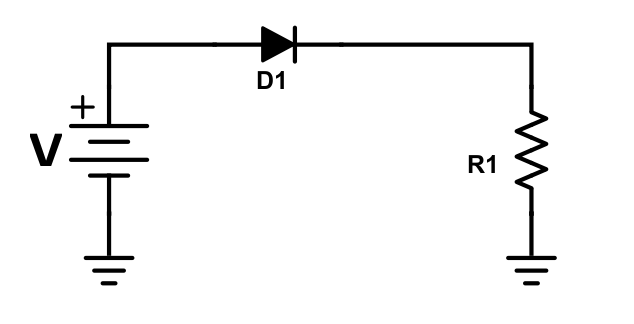
\includegraphics[width=\textwidth]{L1F1.png}
\centering
\end{figure}
The diode behaved as expected based on theory.  At very low voltages a significant portion of the circuit voltage dropped across the diode as the diode contributed a significant amount of the circuit's resistance.  As the applied circuit voltage increased the voltage across the diode leveled off at approximately 0.7V and the majority of the voltage dropped across the resistor.  The current vs. voltage graph of the forward biased diode shows the characteristic nonlinear relationship between current and voltage for this component. 

The second section of the experiment was the analysis of the circuit of figure two, consisting of a reverse biased diode in series with a resistor.  Again a $1k\Omega$ resistor was used for $R_1$ and this time voltages of 0V, 1V, 2V, 5V, 10V, and 15V were applied across the circuit with the voltage across the diode and the current through the diode recorded at each of the input voltages, with the results summarized in Table two in the appendix.  Figure 5 in the appendix is a graph of the data in Table two showing the relationship between current and voltage in this circuit.

\begin{figure}[H]
\caption{Reverse biased diode}
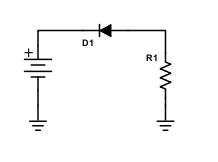
\includegraphics[width=\textwidth]{L1F2.png}
\centering
\end{figure}
Again the diode acted as expected based on theory.  The diode is essentially nonconducting for voltage applied in reverse across its terminals.  The entire applied voltage dropped across the diode and no measurable current was able to flow in the circuit, regardless of the applied voltage.

The third section of the experiment involved the practical analysis of a circuit containing several resistors and diodes.  The circuit analyzed is depicted in Figure three, consisting of two diodes and two resistors.  The applied voltage was 12V, $R_1$ was $10k\Omega$, and $R_2$ was $4.7k\Omega$.  Four different variations of the circuit were analyzed with variation one being the circuit as depicted in Figure three, variation two being the circuit in Figure three except with the orientation of D1 reversed, variation three being the circuit in Figure three except with D2 reversed, and variation four being the circuit in Figure three except with D1 and D2 reversed.  
\begin{figure}[H]
\caption{Practical Analysis of Circuit with PN Diodes}
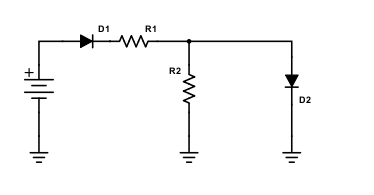
\includegraphics[width=\textwidth]{L1F3.png}
\centering
\end{figure}
The theoretical analysis of the circuit used 0.7V as an approximation for the forward bias potential and an open circuit as a substitute for a reverse biased diode. Variations two and four were straightforward since D1 was reverse biased, all of the applied voltage was predicted to drop across D1  and none across $R_1$ or $R_2$.  

In variation one both diodes were forward biased, so it was predicted that 0.7V would drop across both D1 and D2.  Since $R_2$ is connected in parallel with D2 this meant that the voltage across $R_2$ would be 0.7V as well.  Then applying Kirchoff's voltage law to the loop containing the voltage source and both resistors meant that since 12V was applied to the circuit, 0.7V dropped across D1 and 0.7V dropped across $R_2$, the voltage across $R_1$ had to be $12V-0.7V-0.7V=10.6V$.

In variation three D1 is forward biased but D2 is reverse biased.  The analysis is the same as the analysis of a series circuit with the branch containing D2 removed.  Since 12V was applied to the circuit and 0.7V drops across the forward biased D1, 11.3V would be divided between $R_1$ and $R_2$.  So the voltage across $R_1$ was predicted to be $11.3V\cdot \frac{10k\Omega}{10k\Omega +4.7k\Omega}=7.687V$.  The remaining 3.613V was predicted to drop across $R_2$.

When the circuit of Figure three was constructed and the voltage across each resistor was measured for each variation of the circuit the results agreed closely with the theoretical values.  The values of the theoretically predicted voltage drops across the resistors, measured voltage drops across the resistors, and percent deviation of these two measurements from their theoretical values.  Note, percent deviation was not calculated variations two and four because the theory predicted a drop of 0V across each resistor and percent deviation was calculated as $\frac{V_{measured}-V{theory}}{V_{theory}}$ which is undefined when the theory predicts a drop of 0V.

\section*{Conclusion}
This lab experiment demonstrated the role diodes play in DC circuits and their characteristics when either forward biased or reverse biased.  As predicted by theory approximately 0.7V dropped across forward biased diodes regardless of the voltage applied as long as the applied voltage was not extremely small.  Reverse biased diodes were confirmed to act approximately as open circuits regardless of the amount of voltage applied across them.  Theory predicts that if a large enough voltage were applied across a reverse biased diode it would begin to conduct due to either avalanche breakdown or Zener breakdown, however this was not explored in this experiment.
\pagebreak
\section*{Appendix}
\begin{table}[H]
\caption{V and I for the circuit in Figure 1}
\begin{center} $\begin{tabular}{|c"c|c|} \hline
\text{V(volts)} & V_D(volts) & I_D(milliAmps) \\ \thickhline
0 & 0.0016 & 0 \\ \hline
0.5 & 0.457 & 0.029 \\ \hline
1 & 0.578 & 0.406 \\ \hline
2 & 0.639 & 1.351 \\ \hline
4 & 0.686 & 3.321 \\ \hline
6 & 0.713 & 5.312 \\ \hline
8 & 0.732 & 7.318 \\ \hline
10 & 0.747 & 9.331 \\ \hline
\end{tabular}$\end{center}
\end{table}
\begin{figure}[H]
\caption{Graph of Data in Table 1}
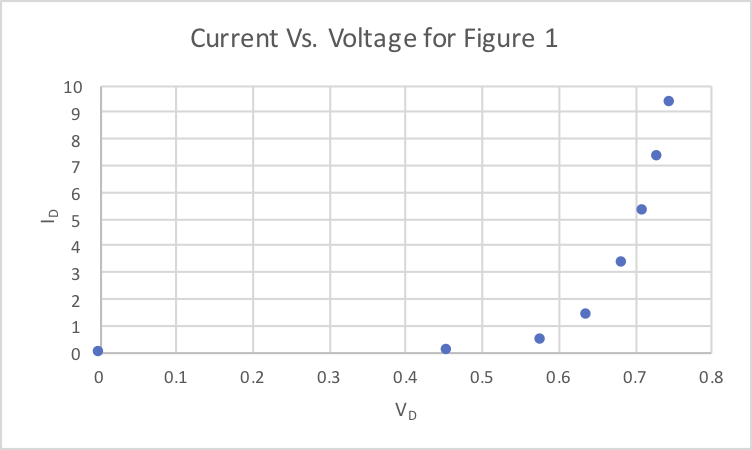
\includegraphics[width=\textwidth]{L1G1.png}
\end{figure}
\begin{table}[H]
\caption{V and I for the circuit in Figure 2}
\begin{center} $\begin{tabular}{|c"c|c|} \hline
\text{V(volts)} & V_D(volts) & I_D(milliAmps) \\ \thickhline
0 & 0.0011 & 0 \\ \hline
1 & 0.980 & 0 \\ \hline
2 & 1.978 & 0 \\ \hline
5 & 4.979 & 0 \\ \hline
10 & 9.975 & 0 \\ \hline
15 & 14.974 & 0 \\ \hline
\end{tabular}$\end{center}
\end{table}
\begin{figure}[H]
\caption{Graph of Data in Table 2}
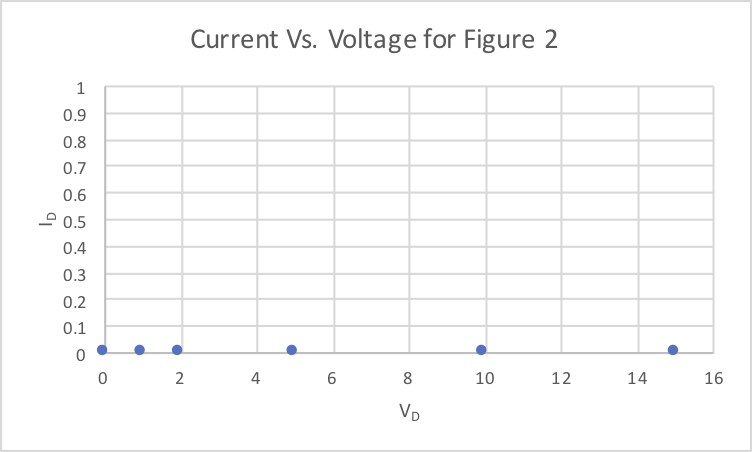
\includegraphics[width=\textwidth]{L1G2.png}
\end{figure}
\begin{table}[H]
\caption{Theoretical and Measured Voltage Drops for the Circuit in Figure Three}
\begin{center}$\begin{tabular}{|c"c|c|c|c|c|c|} \hline
\text{Variation} & V_{R_1 Theory}(V) & V_{R_2 Theory}(V) & V_{R_1 Exp}(V) & V_{R_2 Exp}(V) & \text{\%Dev }V_{R_1}(\%) & \text{\%Dev }V_{R_2}(\%) \\ \thickhline
1 & 10.6 & 0.7 & 10.7 & 0.609 & 0.934 & 13 \\ \hline
2 & 0 & 0 & 0.0001 & 0.00004 & n/a & n/a \\ \hline
3 & 7.687 & 3.613 & 7.669 & 3.690 & 0.234 & 2.13 \\ \hline
4 & 0 & 0 & 0.000005 & 0.000045 & n/a & n/a \\ \hline
\end{tabular}$ \end{center}
\end{table}
\end{document}
